\headline{{\textbf{\Large\sffamily Wired for Bonsai}}\\
          {\textbf{\large\sffamily YouTube Creators Off\--Camera \& Unfiltered}}}
\label{2025-03-wired}
\noindent
Welcome to the first edition of \emph{Wired for Bonsai}, a new feature where we step behind the screen to get to know the personalities shaping the online bonsai world.
In today's fast\--paced digital age, YouTube creators and other online influencers play a huge role in spreading the love for bonsai.
They inspire, educate, and entertain thousands, but what drives them?
What's their own relationship with bonsai beyond the camera?

Each month, we'll sit down with a different creator to hear their unfiltered thoughts on bonsai, their journey, and what keeps them passionate about this art form.

For our very first feature, we're thrilled to chat with \textbf{Andy}, a.k.a. \textbf{Bonsai Crazy}.
Based in London---though on the other side of town from our club---Andy has quickly climbed the ranks of the UK bonsai scene with his unconventional approach and boundless creativity.
His engaging videos have captured the attention of enthusiasts across the country, and soon, his work will be on display at the newly established \emph{Bonsai\--Fest} in Newark, replacing the well-known Doncaster Bonsai Experience.

Let's dive in and get to know Andy beyond the YouTube lens!

\medskip
\topic{Getting to Know Andy and His Bonsai Journey}
\noindent
Andrew Smith, better known as \emph{Bonsai Crazy}, hails from Romford, Essex.
After meeting his girlfriend 22 years ago, he moved to Blackheath in Greenwich, London, where he runs his own window\--cleaning business.
But outside of work, bonsai has become his true obsession.

\emph{``I first started bonsai five years ago after being given a ficus tree from IKEA. It sparked something in me,''} he recalls.
With an addictive personality, Andrew had previously been deeply into carp fishing, but bonsai quickly took over.
\emph{``Bonsai gives me a sense of freedom. It calms me, makes me more aware of nature, and teaches me patience.''}

\begin{window}[%
    2,l,%
    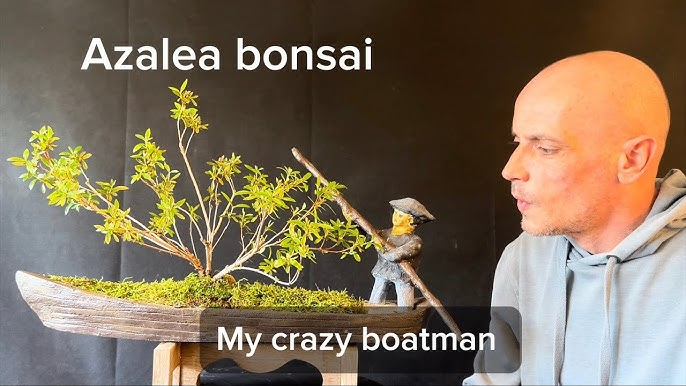
\includegraphics[width=1.0\columnwidth]{2025_03/res/wired_bonsai_crazy},%
    \centerline{\emph{Andy with his Azalea bonsai in his signature `boatman' pot.}}%
]
\end{window}
\columnbreak

His favourite species to work with right now is Japanese larch.
\emph{``Because I'm still a beginner, I love how fast it grows, how flexible it is, and how forgiving it can be when I make mistakes.''}
When asked about his least favourite part of the process, he admits, \emph{``Taking wire off---I find it nerve\--racking!''}
But despite that challenge, it's the creativity of bonsai that keeps him hooked.
\emph{``You have to let your creative juices flow. If you get it wrong, don't worry---you can always find another way to style the tree!''}

As for inspiration, Andrew looks to the trees themselves.
\emph{``Going to bonsai shows and seeing magnificent trees in person is something you can't understand until you stand in front of them.''}
He also follows big names in the bonsai world, including \href{https://www.youtube.com/@EiseienBonsai}{\emph{Bjorn Bjorholm} (Eisen-En Bonsai)}, \href{https://www.youtube.com/@BonsaiMirai}{\emph{Ryan Neil} (Bonsai Mirai)}, and \href{https://www.youtube.com/channel/UClhxFl5LJ8S9j01JV4QMpbw}{\emph{Xavier}'s Bonsai Retreat}.
Closer to home, he has high praise for
\href{https://www.youtube.com/@houghtonbonsai}{\emph{Ryan}} from \href{https://www.youtube.com/@houghtonbonsai}{Houghton Bonsai}, saying, \emph{``He does amazing work with both starter and finished trees. He's definitely worth following!''}

\medskip
\topic{The Bonsai Crazy YouTube Channel}
\noindent
Andrew's \href{https://www.youtube.com/results?search_query=bonsai+crazy}{YouTube channel}, \emph{Bonsai Crazy}, started out as a way to make some extra income---but it quickly became something much bigger.
\emph{``It's like being in a huge club of likeminded people who all love bonsai. Thanks to YouTube, I now have friends all over the world---from Australia to Italy, Spain, France, America, and Canada. It's unbelievable how much it can change your life!''}

On his channel, Andrew shares a mix of bold styling experiments, unique DIY bonsai pots, and hands\--on creative projects.
\emph{``I love transforming raw nursery stock into bonsai and pushing the boundaries with unconventional techniques like root\--over\--rock and tanuki,''} he explains.
His channel also features visits to bonsai nurseries and events, along with community\--focused content where he shares his thoughts on bonsai philosophy.
\emph{``For me, it's all about creativity---bonsai should be fun, and there's no need to stick rigidly to tradition. Just go for it!''}

His hope for his videos is simple: \emph{``I want people to feel part of a community and to have the courage to be creative.
Don't be scared---just go for it!''}

\begin{window}[%
    2,l,%
    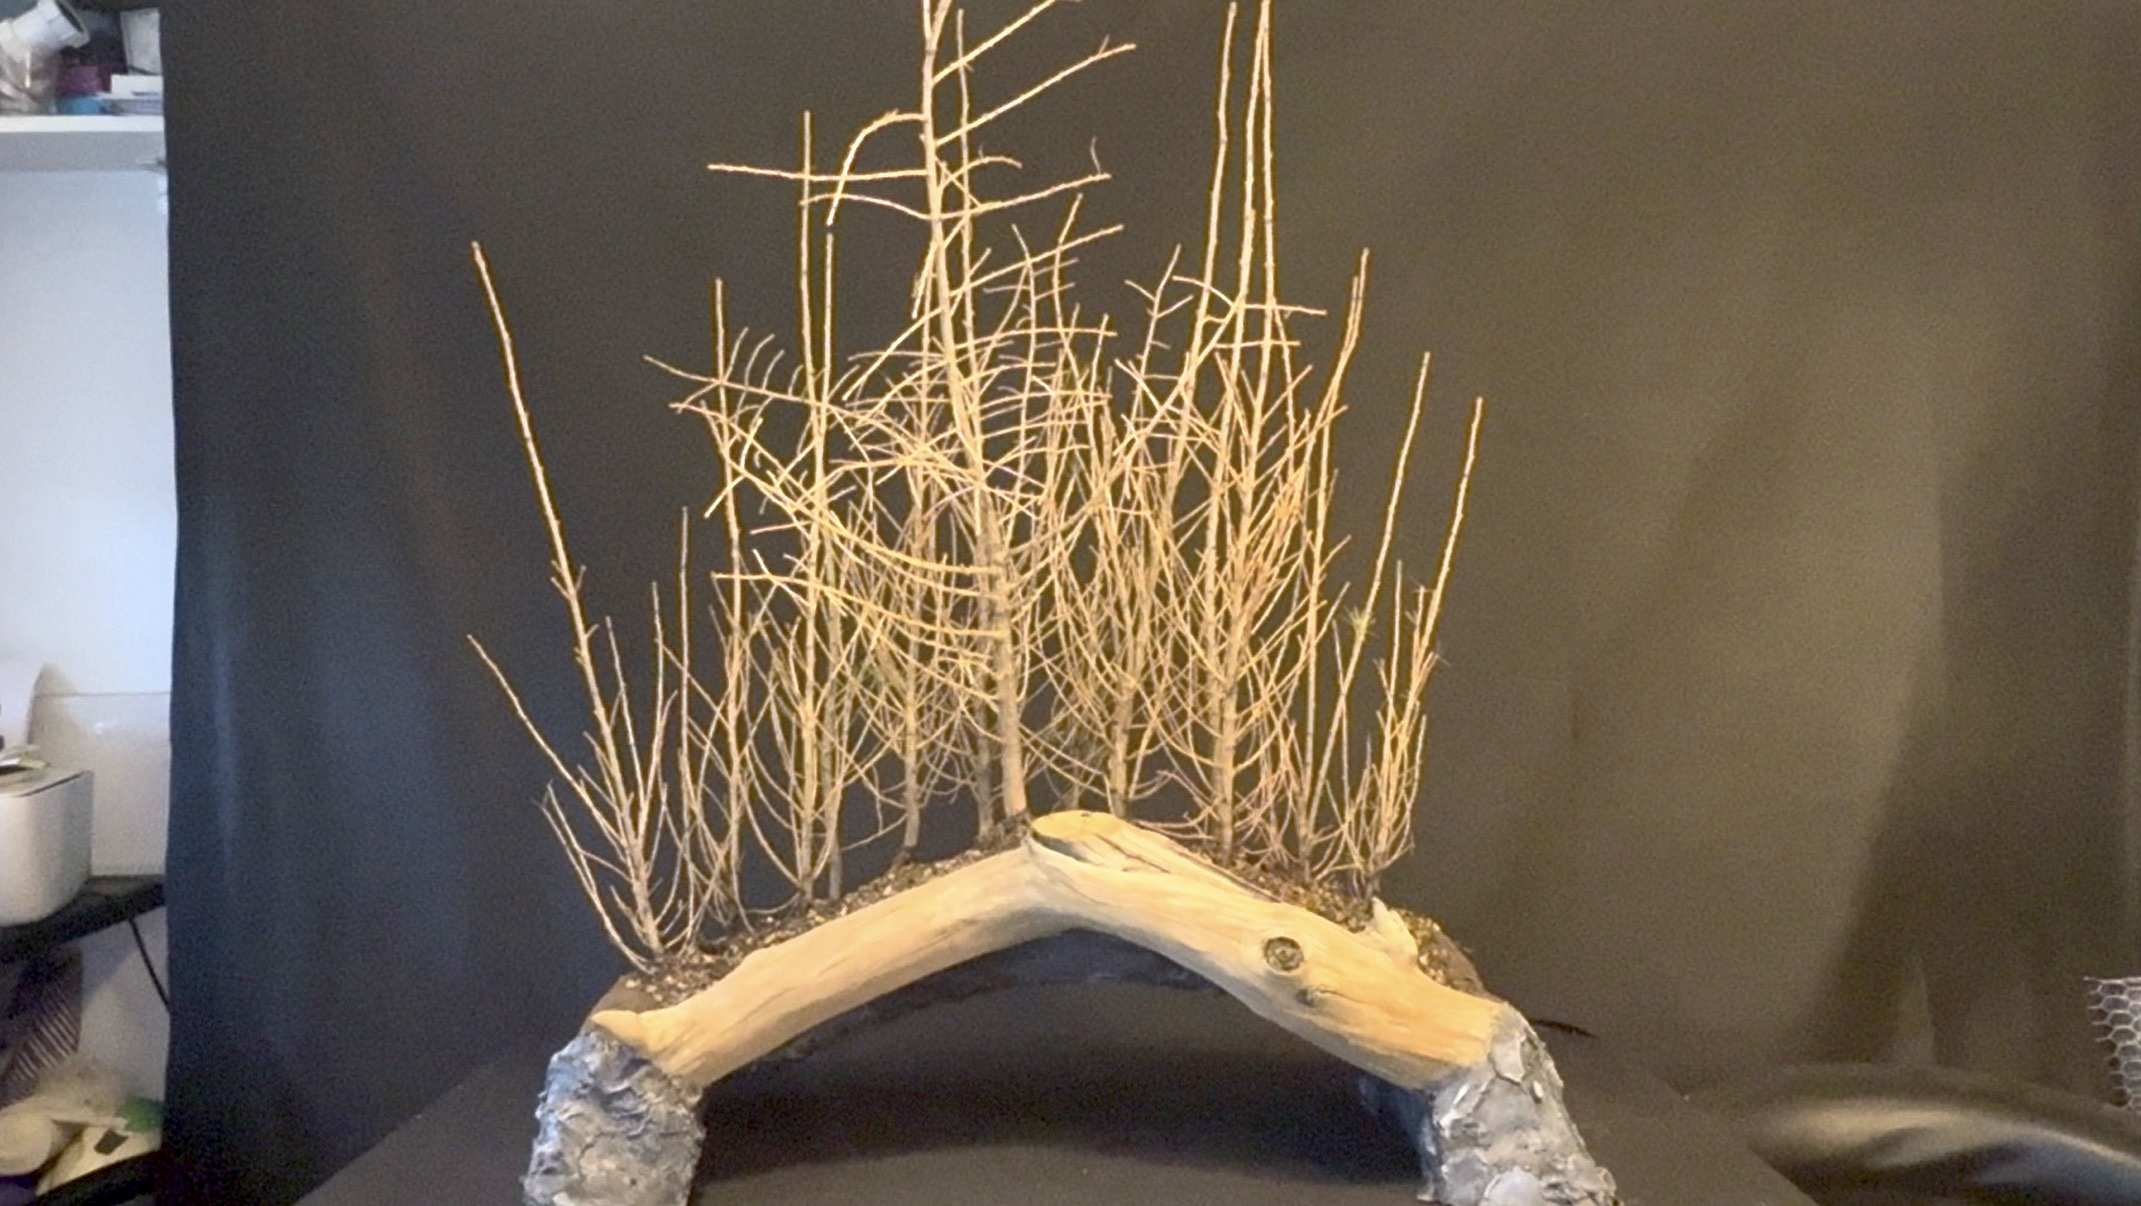
\includegraphics[width=1.0\columnwidth]{2025_03/res/wired_larch_forest},%
    \centerline{\emph{Andy's stunning hillside larch forest in a handcrafted pot.}}%
]
\end{window}
\columnbreak

One of his most memorable videos was the day he met \href{https://www.youtube.com/results?search_query=herons+bonsai}{\emph{Peter Chan}} and discovered the true cost of bonsai.
\emph{``I'll never forget that day,''} he laughs.
\emph{``And I don't need to explain why people connected with it---that's self\--explanatory!''}

Through creating content, Andrew has been surprised by the kindness of the bonsai community.
\emph{``When you get things wrong, people don't tear you down---they help you out!''}
For those thinking about starting a bonsai YouTube channel, he offers this advice: \emph{``Remember, at first, people don't care about you. They care about what you're teaching them. Your personal story comes later---once you've built trust, like Ryan Neil or Bjorn.''}

\medskip
\topic{A Peek into Andy's Bonsai Garden}
\noindent
Andrew has several exciting projects underway, with one standout piece being his \emph{rhino bonsai pot}, featuring a Japanese larch growing from the horn of a custom\--made rhino sculpture.
Another major undertaking is his waterfall root\--over\--rock bonsai, alongside multiple tanuki projects.

When asked about his favourite tree, he names his multi\--trunk thuja.
\emph{``It's an impressive tree that I hope will make it to a show soon. I actually saved it from a customer's garden, and it's only just beginning its bonsai journey.''}
Looking ahead, he's eager to refine his skills.
\emph{``I'd love to try a thread graft or a simple graft sometime soon!''}

\medskip
\topic{Bonsai\--Fest --- The Big Event}
\noindent
\emph{Bonsai\--Fest} marks a major milestone for Andrew---it's the first time he'll be involved in an event as a vendor.
\emph{``I'll be selling my bespoke, handcrafted bonsai pots. They're made from wood and ciment fondu, and they're incredibly unique. You know those pots you see in pictures and think, `Wow, I need that'? Well, I make those!''}

But for Andrew, the real highlight isn't just selling his work---it's meeting his subscribers.
\emph{``I'm most excited to see everyone in person and have a laugh with them.''}
And as for \emph{Bonsai\--Fest's} future?
\emph{I really hope it's a complete success and continues for many years. I can't wait for the weekend!''}

The event is also a huge honour for our club, as the organisers have asked our chairman, Tony Ulatowski, to exhibit one of his trees.
A delegation of members will be heading to Newark to support him and celebrate this special moment.

\begin{window}[%
    2,l,%
    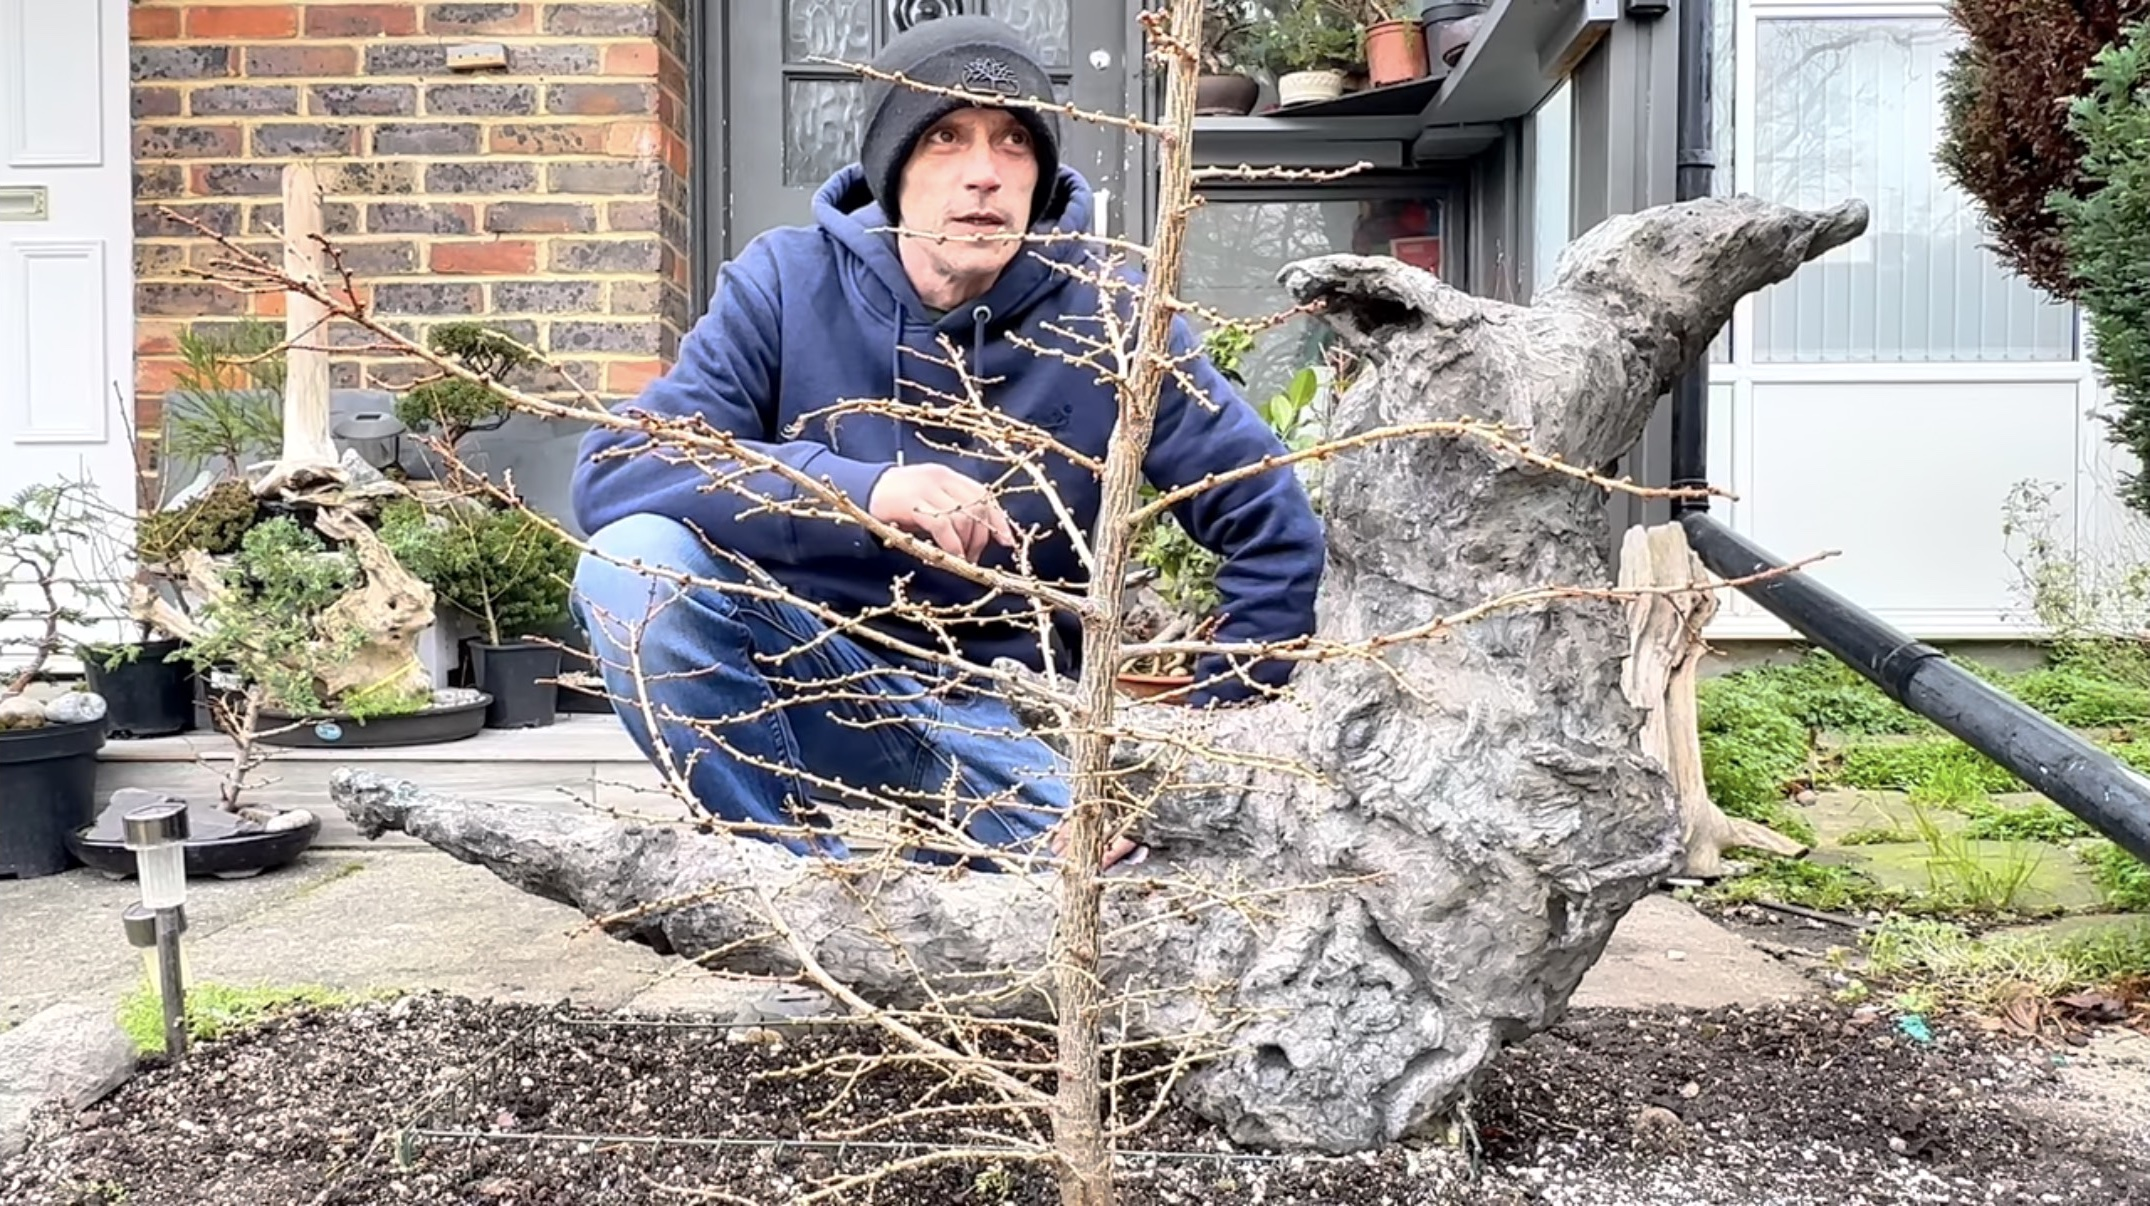
\includegraphics[width=1.0\columnwidth]{2025_03/res/wired_rhyno_pot},%
    \centerline{\emph{Andy with his iconic rhino pot, preparing to plant a tree.}}%
]
\end{window}
\columnbreak

\medskip
\topic{The Future --- What's Next?}
\noindent
Looking ahead, Andrew hopes to keep expanding both his bonsai collection and his YouTube channel.
\emph{``I want to keep pushing myself creatively and learning new techniques.''}
For the UK bonsai scene, he hopes for more community\--driven events and even stronger connections between enthusiasts.

His advice to beginners?
\emph{``Just start. Don't overthink it, don't be afraid---just get stuck in and enjoy the process!''}

His next major project is an experiment to grow the distinctive `knees' of a bald cypress tree---a challenge that has fascinated many bonsai artists.
To support this unique endeavour, he has also created a bespoke pot specifically designed for the project.

\medskip
\topic{Bonsai Clubs --- Community \& Connection}
\noindent
While Andrew has only recently joined a bonsai club, he certainly sees their value.
\emph{``I love the idea of clubs bringing people together. If I were to join one, I'd want it to be a place where people feel encouraged to try new things and experiment with their trees.''}

Andrew is now a member of the \href{https://www.leatherhead-bonsai-club.co.uk}{Leatherhead Bonsai Club}, having joined just two months ago.

And does he have any words for the Twickenham Bonsai Club?
\emph{``Just keep doing what you're doing---spreading the love for bonsai and building a strong community. That's what matters most!''}

\begin{center}
    $\cdots$
\end{center}

We hope you've enjoyed this deep dive into Andy's bonsai journey and the story behind \emph{Bonsai Crazy}.
It's been fantastic getting to know him beyond the screen, and we can't wait to see what he shares with the bonsai world next.

We also wish him the very best for his showcase at \emph{Bonsai\--Fest} at Lady Eastwood Centre in Newark on Sunday 16 March 2025---an exciting milestone for both him and the UK bonsai scene.
If you're attending, be sure to stop by his table, say hello, and check out his unique creations.

And Andy, since we're not that far apart, we'd love to hear all about your \emph{Bonsai\--Fest} experience and maybe even see you in person at our next \emph{Summer Show} in Twickenham.
Until then, happy bonsai!
\closearticle

\begin{window}[%
    2,l,%
    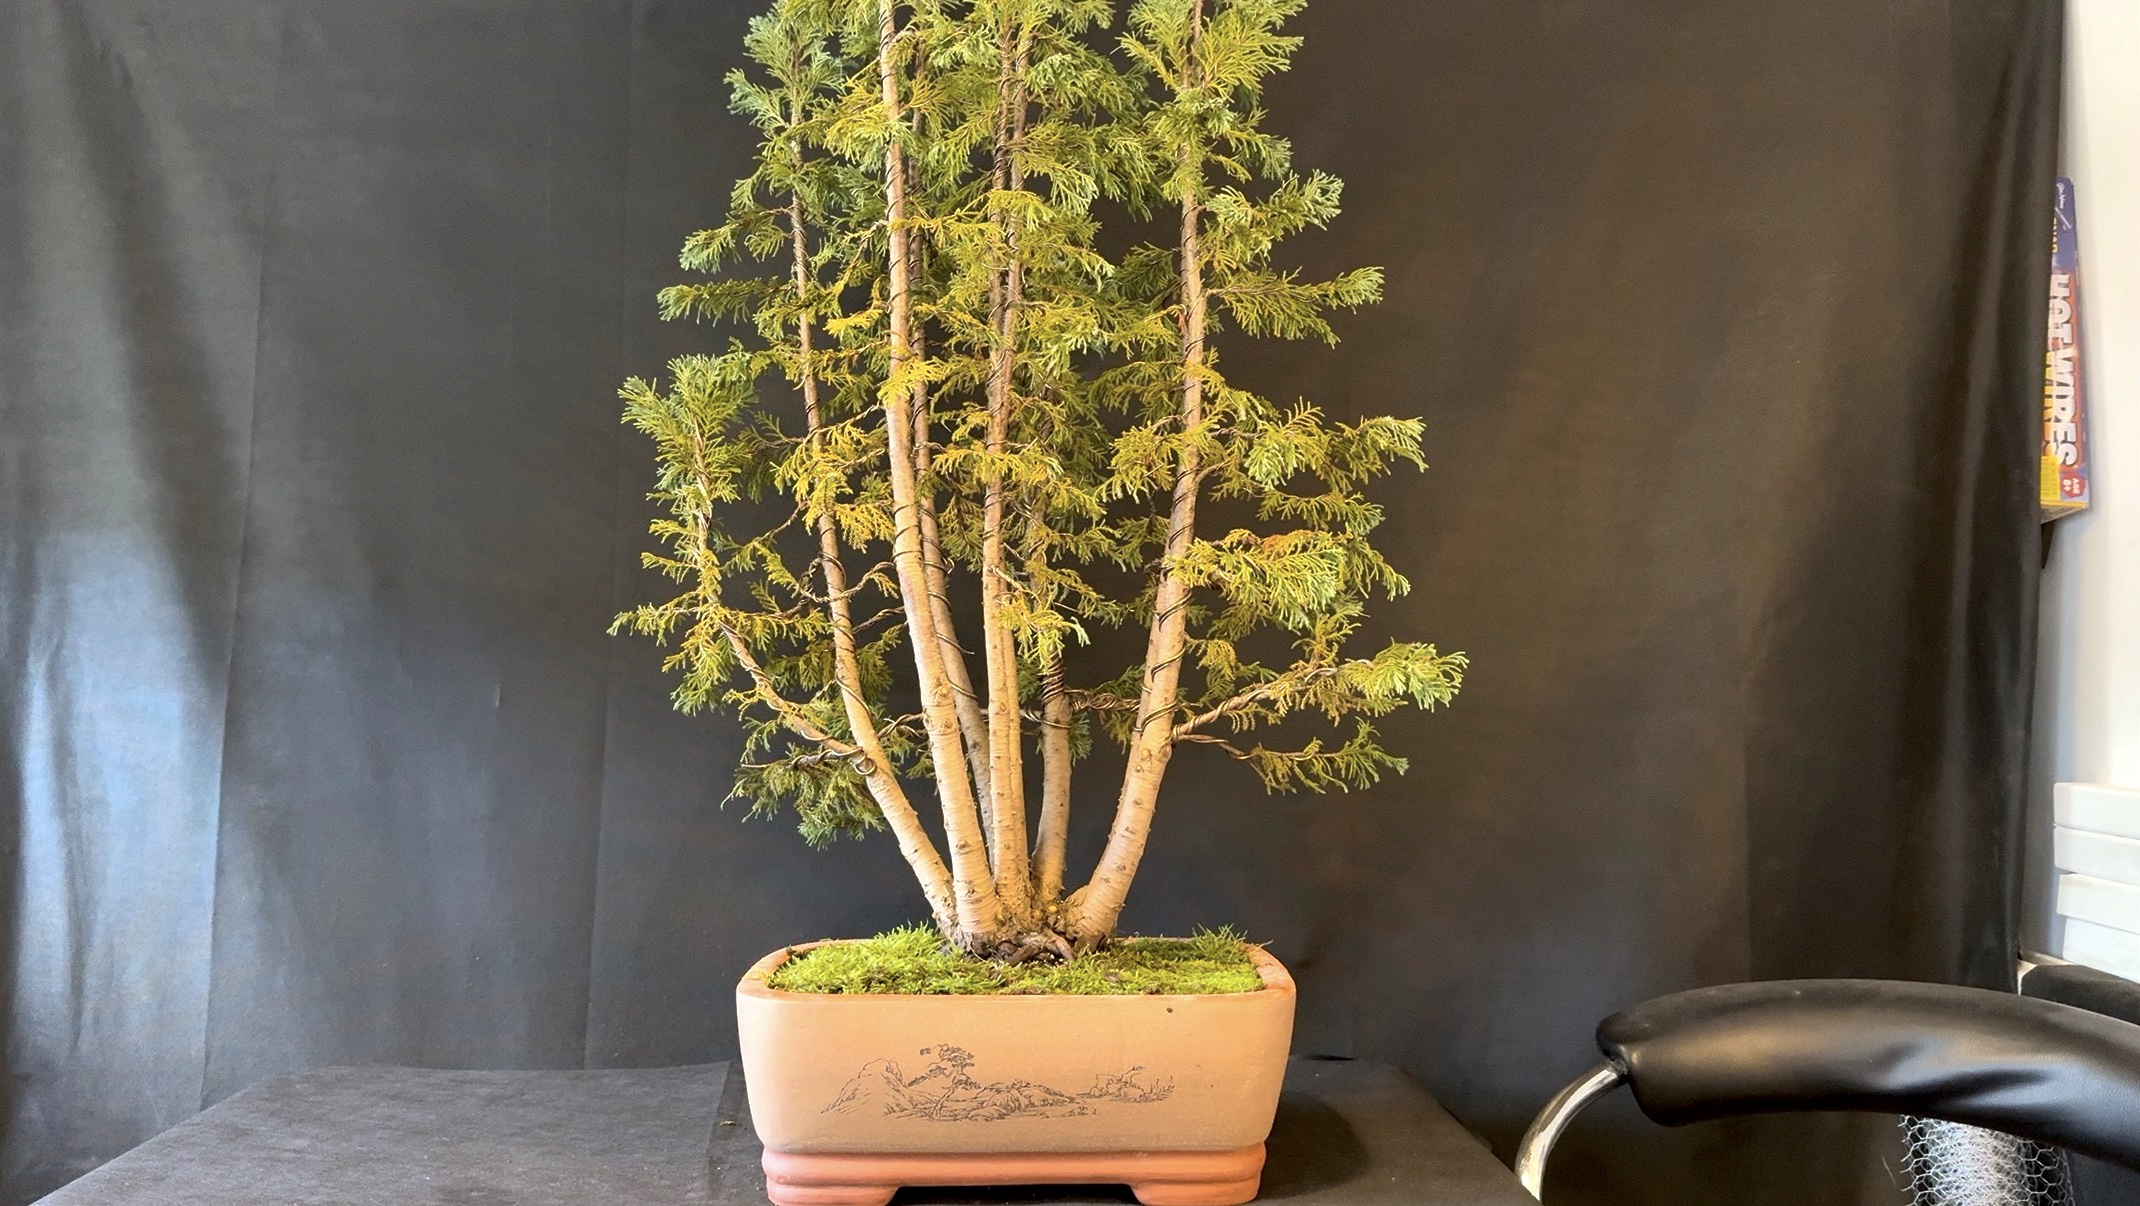
\includegraphics[width=1.0\columnwidth]{2025_03/res/wired_clump_forest},%
    \centerline{\emph{Andy's charming clump forest, truly a natural tiny beauty.}}%
]
\end{window}
\columnbreak
